\chapter{Planteamiento}
\section{Sistema}
Lo que se busca es simular un sistema \gls{dtfm} cuya señal se transmite a través de un canal telefónico con modulación \gls{am}. Tal simulación debe comprender cada uno de los bloques intervinientes en el sistema, como se muestra en la Figura \ref{fig:diagrama_bloques_objetivo}. Antes de diseñar y planificar la simulación hay que tener en cuenta las frecuencias intervinientes, particularmente hablando de la \gls{fp} (que determina la frecuencia de la señal a ser modulada en la transmisión) y la \gls{fs} (que determina la cantidad de muestras por segundo para la simulación).

Ya que esta simulación trata de la transmisión en \gls{am} a través de un canal telefónico, podemos tomar una \gls{fs} utilizada universalmente en sistemas de audio, y esta equivale a 44 [kHz], y podemos ver que claramente cumple con el Teorema de Nyquist-Shannon ya que es mayor al doble de la señal de mayor frecuencia (1477 [Hz], componente alta de los digitos 3, 6 y 9). Para la \gls{fp} tomamos 15 [kHz] ya que es 10 veces mayor a la señal antes mencionada y es menor a la mitad de \gls{fs} (para poder seguir cumpliendo con el teorema).

A continuación enumeramos el tratamiento de la señal en cada bloque del sistema:

\begin{enumerate}
  \item Codificador DTMF: Se suman las señales sinusoidales correspondientes a las frecuencias que componen cada digito
  \item Modulador AM: Se modula la señal portadora con la señal codificada
  \item Cable Telefónico: La señal modulada pasa por un filtro pasa-banda para simular el canal de voz [300-3300][Hz]
  \item Demodulador AM: Se bate la señal recibida con la misma portadora para obtener la moduladora
  \item Decodificador DTMF: La señal pasa por un banco de filtros pasa-banda para determinar qué señales de la matriz fueron enviadas
\end{enumerate}

\begin{figure}[H]
  \centering
  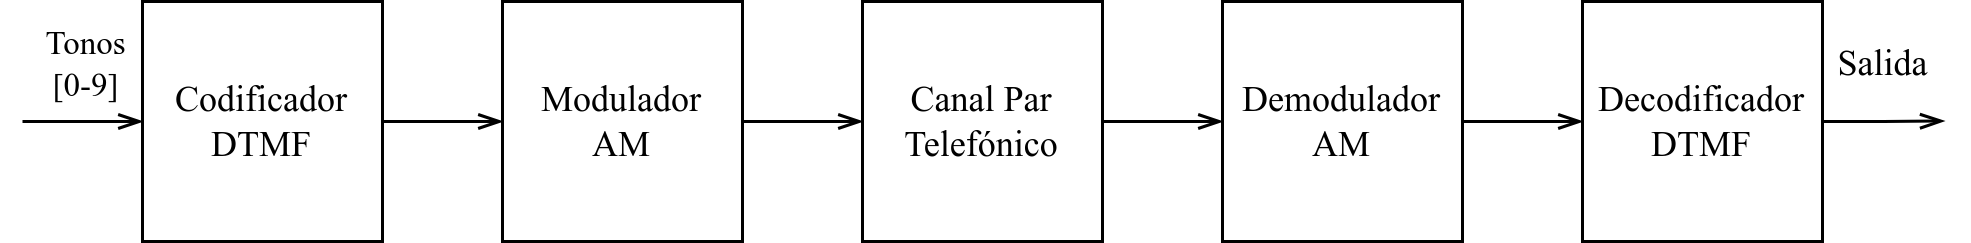
\includegraphics[width=\linewidth]{images/planteamiento/bloques.png}
  \caption{Diagrama de bloques a simular}
  \label{fig:diagrama_bloques_objetivo}
\end{figure}

\section{Decodificación}
Para decodificar la señal del tono se tiene que implementar un banco de filtros en base a la matriz de señales del sistema \gls{dtfm}. Esto es, las filas se corresponden con las frecuencias bajas y las columnas con las frecuencias altas. La sumatoria de las señales se corresponde con la codificación del tono propuesto; esta señal llega a la matriz para devolver el tono correspondiente. El bloque decodificador se compone de filtros pasa-banda para cada frecuencia y el bloque detector como muestra la Figura \ref{fig:diagrama_bloques_decod}. La razón de usar un filtro para cada frecuencia baja y alta, en lugar de un filtro por cada frecuencia resultante, se debe a que de esta forma usamos 7 filtros en lugar de 9 (uno por cada tono); además, estas frecuencias (altas y bajas) están más separadas en el espectro que las frecuencias resultantes, lo cual es provechoso a la hora de diseñar un filtro.

La matriz será un bloque lógico que devolverá el digito correspondiente en base a las señales que hayan logrado activarse luego pasar por el banco de filtros.

\begin{figure}[H]
  \centering
  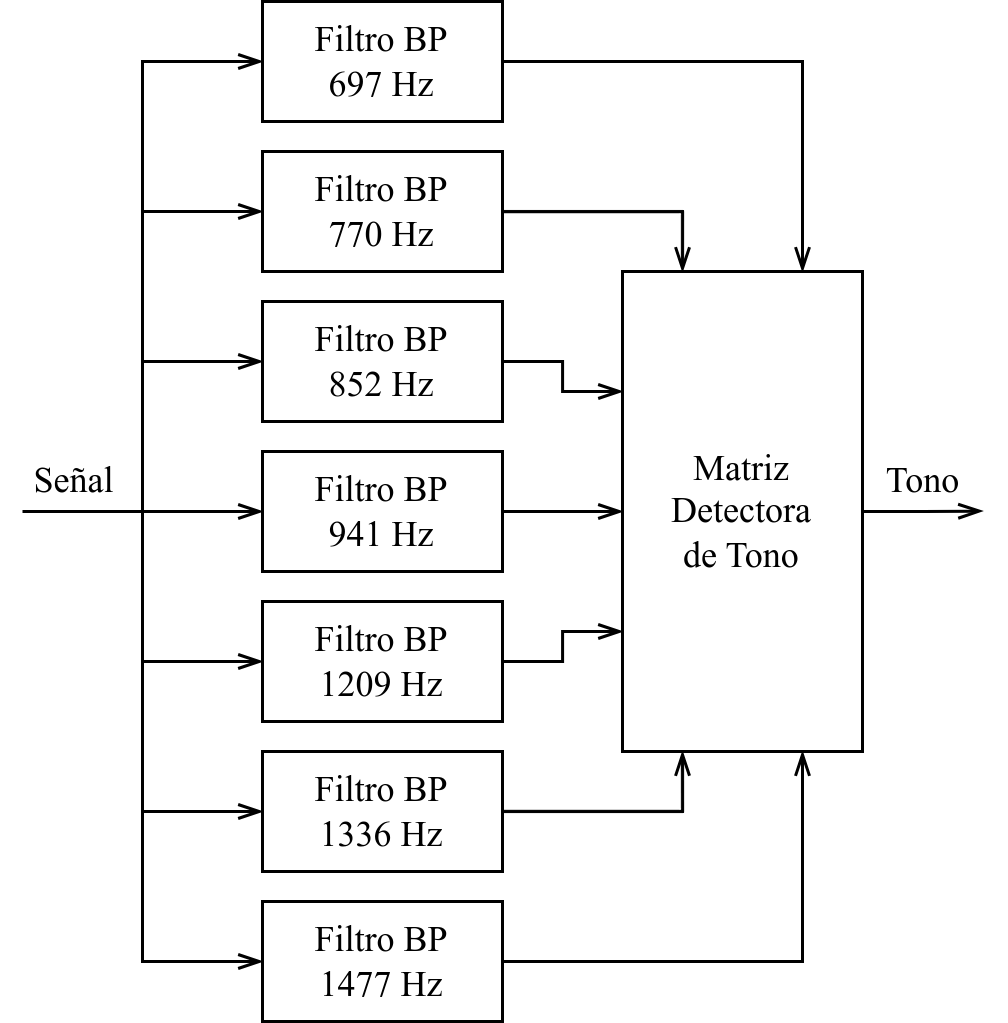
\includegraphics[width=300pt]{images/planteamiento/decodificador.png}
  \caption{Composición del bloque decodificador}
  \label{fig:diagrama_bloques_decod}
\end{figure}

\section{Simulación}
La simulación de este sistema, que es el objetivo de este proyecto, se logrará a través del uso de distintas herramientas dentro del software MATLAB. Entre estas herramientas se encuentra simulink que sirve para realizar el estudio en el tiempo y frecuencia de las señales a través de cada bloque del sistema.

Cada señal de entrada al sistema será simulada a través de generadores de sinusoidales, mientras que los filtros serán bloques que actuen en base a polinomios obtenidos por librerías provistas por MATLAB. El resto de las herramientas serán provistas por simulink (sumadores, multiplicadores, analizadores de espectro, etc.)

La razón de usar una herramienta para el diseño de los filtros es que estos se presumen de alto orden, lo cual es engorroso de calcular de manera analítica. Sin embargo, con el objetivo de comprender cómo es el diseño de filtros digitales, se explicará en el siguiente capítulo cómo es el proceso de diseño y análisis correspondiente.